% !TeX encoding = UTF-8
% !TeX program = lualatex
% !TeX spellcheck = en_US

% An alternative to the following \documentclass is
% \documentclass{beamer}
% \mode<presentation>
% {
%   \usetheme{default}
%   \setbeamercovered{transparent}
% }

\documentclass[presentation,english,aspectratio=169]{beamer}

% Remove the annoying symbols no one uses anyway.
\beamertemplatenavigationsymbolsempty

% Most of these were autogenerated by org export to beamer.tex file
% I don't know if they are all necessary, but I don't think there is any harm in
% including them.
\usepackage[utf8]{luainputenc}
%\usepackage[T1]{fontenc} %MK: LuaLaTeX only properly supports unicode fonts ("TU")

\usepackage{graphicx}
\usepackage{grffile}
\usepackage{longtable}
\usepackage{wrapfig}
\usepackage{rotating}
\usepackage[normalem]{ulem}
\usepackage{amsmath}
\usepackage{textcomp}
\usepackage{amssymb}
\usepackage{capt-of}
\usepackage{hyperref}
\usetheme{default}

% I'm not sure what exactly this is for
% It is copied from a template provided by Till Tantau
% <tantau@users.sourceforge.net>
%\usepackage[english]{babel} %MK: for LuaLaTeX, use polyglossia (if needed)

% It is copied from a template provided by Till Tantau
% <tantau@users.sourceforge.net>
% I'm not sure what exactly this is for
%\usepackage{times} %MK: Not available for unicode fonts (it's a Type-1 font, obsolete and its maintainer is dead); use \uspackage{fontspec} to customize font.

\usepackage{listings}
\usepackage{xcolor}
\usepackage{minibox}
\usepackage{tikz}
\usetikzlibrary{decorations.text}
\usetikzlibrary{shadows}
\usetikzlibrary{fit}
\usetikzlibrary{graphs}
\usetikzlibrary{graphdrawing}
\usegdlibrary{layered}

\pgfdeclarelayer{backbackbackground}
\pgfdeclarelayer{backbackground}
\pgfdeclarelayer{background}
\pgfdeclarelayer{foreground}
\pgfdeclarelayer{foreforeground}
\pgfsetlayers{backbackbackground,backbackground,background,main,foreground,foreforeground}

\lstset{
  basicstyle=\ttfamily,
  columns=fullflexible,
  breaklines=true,
  postbreak=\raisebox{0ex}[0ex][0ex]{\color{red}$\hookrightarrow$\space}
}

% Use this to adjust text for overlays
% If set to transparent, then text is overlays is visible, but greyed out.
% If not set, then the text in overlays is not visible at all (i.e., invisible).
\setbeamercovered{transparent}

\usecolortheme{}
\usefonttheme{}
\useinnertheme{}
\useoutertheme{}
\author[Author, Another] % {optional, use only with lots of authors
       {Kit Barton\inst{1} \and \\
        Johannes Doerfert\inst{2} \and \\
        Hal Finkel\inst{2} \and \\
        Michael Kruse\inst{2} \and \\
        Ettore Tiotto\inst{1}}

% Give the names in the same order as they appear in the paper.
% Use the \inst{?} command only if the authors have different
% affiliation.
\institute[IBM Canada and ANL] % (optional, but mostly needed)
{
  \inst{1}
  IBM Canada
  \inst{2}
  Argonne National Laboratory
}

% Pick the date.
% Hard code it or pick a floating date based on day the PDF was built.
% Can also be a string
%\date[August 15, 2019]{Name of Conference here}
\date{October 23, 2019}

\title{Writing Loop Optimizations in LLVM}

% Autogenerated by org export to beamer.tex file
\hypersetup{
 pdfauthor={Kit Barton},
 pdftitle={Beamer Template},
 pdfkeywords={},
 pdfsubject={},
 pdfcreator={},
 pdflang={English}}

%\subject{Theoretical Computer Science}
% This is only inserted into the PDF information catalog. Can be left
% out.



% If you have a file called "university-logo-filename.xxx", where xxx
% is a graphic format that can be processed by latex or pdflatex,
% resp., then you can add a logo as follows:

\pgfdeclareimage[height=0.5cm]{ibm-logo}{figures/IBMLogo}
\pgfdeclareimage[height=0.5cm]{anl-logo}{figures/anl-symbol} % MK: Feel free to replace with smaller logo
\logo{\pgfuseimage{anl-logo}\hspace*{.9\linewidth}\pgfuseimage{ibm-logo}}

% Delete this, if you do not want the table of contents to pop up at
% the beginning of each subsection:
%% \AtBeginSubsection[]
%% {
%%   \begin{frame}<beamer>{Outline}
%%     \tableofcontents[currentsection,currentsubsection]
%%   \end{frame}
%% }


% If you wish to uncover everything in a step-wise fashion, uncomment
% the following command:

%\beamerdefaultoverlayspecification{<+->}



\makeatletter
% pgf 'file' shape
\def\myfoldheight{0.5}
\def\myshapepath{
	\pgfextract@process\northwest{
		\southwest\pgf@xa=\pgf@x
		\northeast
		\pgf@x=\pgf@xa
	}

	\pgfextract@process\southeast{
		\southwest\pgf@ya=\pgf@y
		\northeast
		\pgf@y=\pgf@ya
	}

	\pgfextract@process\northfold{
		\pgfpointdiff{\southwest}{\northeast}
		\northeast
		\advance\pgf@x-\myfoldheight\pgf@y
	}

	\pgfextract@process\eastfold{
		\pgfpointdiff{\southwest}{\northeast}
		\northeast
		\advance\pgf@y-\myfoldheight\pgf@y
	}

	\pgfextract@process\fold{
		\northfold\pgf@xa=\pgf@x
		\eastfold
		\pgf@x=\pgf@xa
	}

	\pgfpathmoveto{\southwest}
	\pgfpathlineto{\northwest}
	\pgfpathlineto{\northfold}
	\pgfpathlineto{\eastfold}
	\pgfpathlineto{\southeast}
	\pgfpathclose
}

% compute an intersection point between a line and \myshapepath
% NOTE: Breaks inside \graph[layered layout]
\def\myshapeanchorborder#1#2{
	% #1 = point inside the shape
	% #2 = direction
	\pgftransformreset % without this, the intersection commands yield strange results
	\pgf@relevantforpicturesizefalse % don't include drawings in bounding box
	\pgfintersectionofpaths{
		\myshapepath
		%\pgfgetpath\temppath\pgfusepath{stroke}\pgfsetpath\temppath % draw path for debugging
	}{
		\pgfpathmoveto{
			\pgfpointadd{
				\pgfpointdiff{\southwest}{\northeast}\pgf@xc=\pgf@x \advance\pgf@xc by \pgf@y % calculate a distance that is guaranteed to be outside the shape
				\pgfpointscale{
					\pgf@xc
				}{
					\pgfpointnormalised{
						#2
					}
				}
			} {
				#1
			}
		}
		\pgfpathlineto{#1}
		%\pgfgetpath\temppath\pgfusepath{stroke}\pgfsetpath\temppath % draw path for debugging
	}
	\pgfpointintersectionsolution{1}
}
\def\myshapeanchorcenter{
	\pgfpointscale{.5}{\pgfpointadd{\southwest}{\northeast}}
}

% we could probably re-use some existing \dimen, but better be careful
\newdimen\myshapedimenx
\newdimen\myshapedimeny

\pgfdeclareshape{file}{
	% some stuff, we can inherit from the rectangle shape
	\inheritsavedanchors[from=rectangle]
	\inheritanchor[from=rectangle]{center}
	\inheritanchor[from=rectangle]{mid}
	\inheritanchor[from=rectangle]{base}

	% calculate these anchors so they lie on a coorinate line with .center
	\inheritanchor[from=rectangle]{west}
	\inheritanchor[from=rectangle]{east}
	\inheritanchor[from=rectangle]{north}
	\inheritanchor[from=rectangle]{south}

	% calculate these anchors so they lie on a line through .center and the corresponding anchor of the underlying rectangle
	\inheritanchor[from=rectangle]{south west}
	\inheritanchor[from=rectangle]{south east}
	\inheritanchor[from=rectangle]{north west}
	%    \inheritanchor[from=rectangle]{north east}

	% somewhat more special anchors. The coordinate calculations were taken from the rectangle node
	\inheritanchor[from=rectangle]{mid west}
	\inheritanchor[from=rectangle]{mid east}
	\inheritanchor[from=rectangle]{base west}
	\inheritanchor[from=rectangle]{base east}

	\backgroundpath{
		\myshapepath
	}

	\foregroundpath{
		\pgfpathmoveto{\northfold}
		\pgfpathlineto{\fold}
		\pgfpathlineto{\eastfold}
	}

	% This is from rectangle, i.e. without the fold.
	\anchorborder{%
		\pgf@xb=\pgf@x% xb/yb is target
		\pgf@yb=\pgf@y%
		\southwest%
		\pgf@xa=\pgf@x% xa/ya is se
		\pgf@ya=\pgf@y%
		\northeast%
		\advance\pgf@x by-\pgf@xa%
		\advance\pgf@y by-\pgf@ya%
		\pgf@xc=.5\pgf@x% x/y is half width/height
		\pgf@yc=.5\pgf@y%
		\advance\pgf@xa by\pgf@xc% xa/ya becomes center
		\advance\pgf@ya by\pgf@yc%
		\edef\pgf@marshal{%
			\noexpand\pgfpointborderrectangle
			{\noexpand\pgfqpoint{\the\pgf@xb}{\the\pgf@yb}}
			{\noexpand\pgfqpoint{\the\pgf@xc}{\the\pgf@yc}}%
		}%
		\pgf@process{\pgf@marshal}%
		\advance\pgf@x by\pgf@xa%
		\advance\pgf@y by\pgf@ya%
	}

	%    \anchorborder{
	%        \myshapedimenx=\pgf@x
	%        \myshapedimeny=\pgf@y
	%        \myshapeanchorborder{\myshapeanchorcenter}{\pgfpoint{\myshapedimenx}{\myshapedimeny}}
	%    }
}

\newsavebox{\my@resizeenv@TempBox}%
\newcommand*{\my@resizeenv@width}{}%
\newenvironment{resizeenv}[1]{%
\renewcommand*{\my@resizeenv@width}{#1}%
\begin{lrbox}{\my@resizeenv@TempBox}%
}{%
\end{lrbox}%
\resizebox{\my@resizeenv@width}{!}{\usebox{\my@resizeenv@TempBox}}%
}%

\newenvironment{resizepar}{%
\begin{resizeenv}{\textwidth}%
}{%
\end{resizeenv}%
}%
\makeatother


\begin{document}

% Create the title page
\begin{frame}
  \titlepage
\end{frame}

% Create an outline slide
\begin{frame}{Outline}
  \tableofcontents
  % You might wish to add the option [pausesections]
\end{frame}

% Create a section; comment out if not desired.
\section{Terminology}
\label{sec:terminology}

\begin{frame}[label={sec:org8787e08}]{Loop Representation in LLVM}

  % KB: I will clean this slide up and make it into a proper beamer slide, with
  % animations, if everyone is OK with how it looks.
  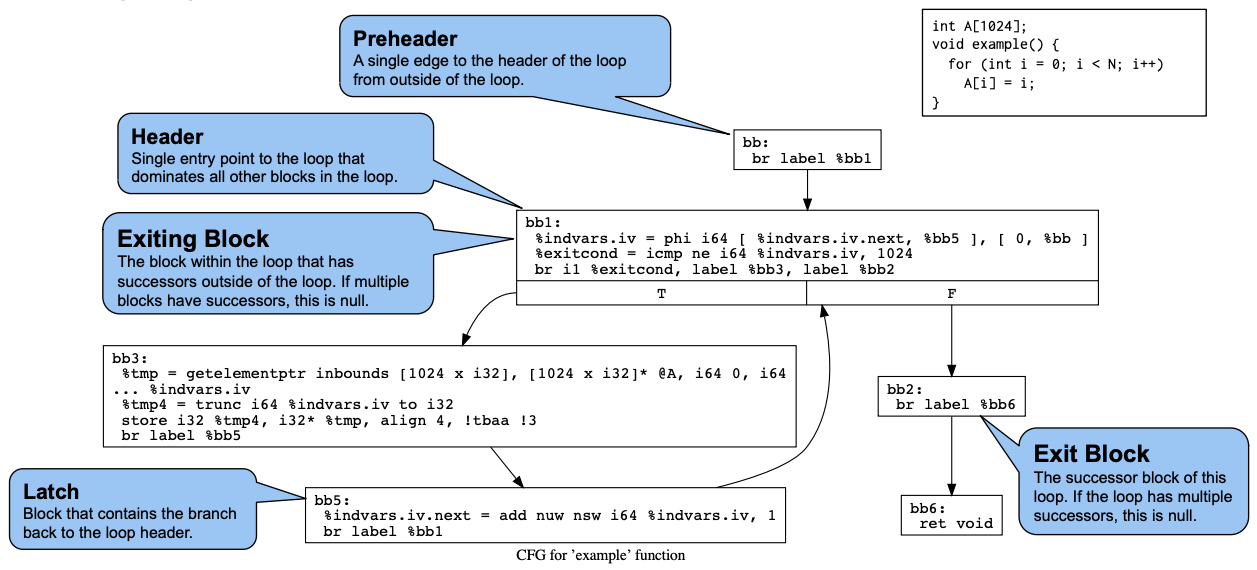
\includegraphics[width=\textwidth]{figures/LoopRepresentation.png}
\end{frame}

\begin{frame}[label={sec:orgac3eb21}]{Other Terminology}
  \begin{block}{}
    \begin{itemize}
    \item Loop predecessor
    \item Backedge taken count
    \item Iteration count
    \item Loop guard
    \item irreducible loops (not covered)
    \item Others?
    \end{itemize}
  \end{block}
\end{frame}

\begin{frame}[label={sec:rotated}]{Rotated Loops}
  \begin{itemize}
    \item Describe what rotated loops are
    \item Give some examples of rotated loops
    \item Limitations of loop rotation
  \end{itemize}
\end{frame}

\begin{frame}[label={sec:canonical}]{Canonical Form}
Describe loop canonical form - what exactly this entails, \textit{etc}.
\end{frame}

\begin{frame}[label={sec:lcssa}]{Loop Closed SSA Form}
% MK: TODO
    What exactly is this? When is it useful? What are the implications afterwards?
\end{frame}

%MK: Not sure whether I am going to need this; for now it's for testing whether tikzpictruew works
\begin{frame}[fragile]{Clang/LLVM/Polly Compiler Pipeline}
\begin{resizepar}
\begin{tikzpicture}
\tikzset{tight/.style={inner sep=0pt,outer sep=0pt,minimum size=0pt}}
\tikzset{node/.style={draw=teal,line width=1.2pt,rounded corners,top color=teal!50,bottom color=white,shading angle=15,drop shadow}}
\tikzset{supernode/.style={subgraph text none,bottom color=teal!30,top color=teal!05,shading angle=15,rounded corners}}
\tikzset{edge/.style={->}}

\graph[layered layout,edges={edge,rounded corners},level sep=5mm,sibling sep=10mm]{
	c[as={\minibox{\texttt{void f() \{}\\\hspace*{4mm}\texttt{for (int i=...)}\\\hspace*{4mm}\dots}},grow=right,draw,shape=file,fill=white,label={source.c}];
	ir[as={IR},shape=file,draw,fill=white,nudge=(up:10mm)];
	asm[as={Assembly},shape=file,draw,fill=white];

	clang [subgraph text none,label={[font=\Large\sffamily]above:Clang}] // [sibling sep=2mm,grow=down,layered layout] {
		lexer [as={Lexer},node];
		parser [as={Parser},node,grow=down];
		preprocessor [as={Preprocessor},node];
		sema [as={Semantic Analyzer},node];
		codegen [as={IR Generation},node];
		%
		lexer->preprocessor->parser->sema->codegen;
	};

	llvm [subgraph text none,label={[font=\Large\sffamily]above:LLVM}] // [sibling sep=2mm,grow=down,layered layout] {
		canonicalization [as={Canonicalization passes},node];
		loopopts [as={Loop optimization passes},node];
		polly [as={Polly},node];
		vectorization [as={LoopVectorize},node];
		latepasses [as={Late Mid-End passes},node];
		backend [as={Target Backend},node];
		%
		canonicalization->loopopts->vectorization->latepasses->backend;
		loopopts->polly->vectorization;
	};

	c->[in=180]lexer;
	codegen->[out=0,in=-90]ir;
	ir->[out=90,in=180]canonicalization;
	backend->[out=0,in=-90]asm;
};

\begin{pgfonlayer}{background}
\node[tight,fit={(clang)},supernode]{};
\node[tight,fit={(llvm)},supernode]{};
\end{pgfonlayer}

%	\path (preprocessor) edge[edge,densely dotted,bend left=50,draw=blue!50!black] node[midway,right,font=\ttfamily,blue!50!black] {\#pragma} (sema);
%	\path (preprocessor) edge[edge,densely dotted,bend right=80,draw=blue!50!black] node[pos=0.7,left,font=\ttfamily,blue!50!black] {\#pragma} (codegen);

	\path (codegen) edge[edge,dashed,bend right=80,draw=blue!50!black,postaction={decorate,decoration={text along path,text={|\color{blue!50!black}|Loop metadata},raise=-1.7ex,pre=moveto,pre length=13mm}}] (ir);
	\path (ir) edge[edge,dashed,draw=blue!50!black] (loopopts);
%	\path (ir) edge[edge,dashed,draw=blue!50!black] (polly);1
	\path (ir) edge[edge,dashed,draw=blue!50!black,bend right=10] (vectorization);
%	\path (polly) edge[edge,dashed,draw=blue!50!black,bend right=10] (vectorization);
\end{tikzpicture}
\end{resizepar}
\end{frame}


\begin{frame}{Current LLVM Loop Optimization Passes}
\end{frame}

\begin{frame}[label={sec:auxdatastruct}]{Auxiliary Data Structures}
    \begin{itemize}
    \item Dominator/PostDominator trees
    \item Data dependence graph (DDG)
    \item Others??
    \end{itemize}
\end{frame}

\section{Considerations when writing a loop pass}
\begin{frame}[label={sec:looppass}]{Loop Pass vs Function Pass}
  \begin{itemize}
  \item What is a loop pass
  \item What is a function pass
  \item Differences/pros/cons of using one over the other
  \end{itemize}
\end{frame}

\begin{frame}[label={sec:passmanager}]{Pass Managers}
  \begin{itemize}
    \item New Pass Manager
    \item Legacy Pass Manager (JD: I would only mention: use the new one)
    \item Where to put loop optimizations in the loop opt pipeline (maybe on new slide)
  \end{itemize}
\end{frame}

\section{Other Useful Tools}
\begin{frame}[label=reports]{Reporting success and failure}
  \begin{itemize}
    \item STATISTICS
    \item Optimization Remark Emitter
  \end{itemize}
\end{frame}

\begin{frame}[label={sec:datastructs}]{Updating Data Structures}
    \begin{itemize}
      \item DominatorTreeUpdater
      \item SCEV
      \item Other??
    \end{itemize}
\end{frame}

\section{Dependence Graphs}
\begin{frame}[label={sec:DepGraphs}]{Dependence Graphs}
  \begin{itemize}
    \item Represents data dependencies between program elements (instructions)
    \item Ideas: 
    \begin{itemize}
      \item D.J. Kuck, R.H. Kuhn, D.A. Padua, B. Leasure, and M. Wolfe (1981). Deendence Graphs and Compiler Optimizations. 
      \item J. Ferrante, K.J. Ottenstein and Joe D. Warren (1987). The Program Dependence Graph and Its Use in Optimizations.
    \end{itemize}
    \item Data Dependence Graph (DDG): hierarchical representation, nodes that are part of an SCC grouped into pi-blocks
    \item Program Dependence Graph (PDG): capable of representing both data dependencies and control-flow dependencies
  \end{itemize}
\end{frame}

\begin{frame}[label=DDGExample1]{Data Dependence Graph Example}
  \begin{itemize}
    \item Example code contains a statement that has a loop carried data dependence on itself
    \item Instructions (nodes) are connected by edges to represent dependencies (def-use and memory)
    \item Def-use relations and a memory access dependency form a cycle representing the loop carried dependence.
  \end{itemize}
  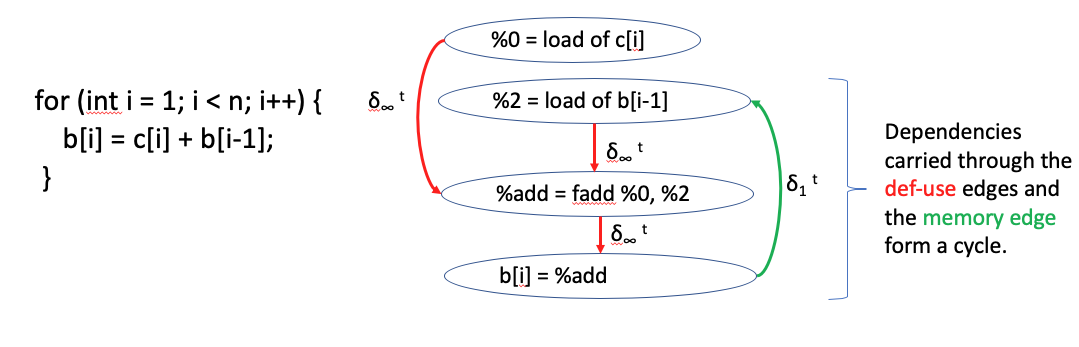
\includegraphics[width=\textwidth]{figures/DDG1.png}
\end{frame}

\begin{frame}[label=DDGExample2]{Data Dependence Graphs Example}
  \begin{itemize}
    \item The DDG corresponding to the example contains a pi-block 
    \item The pi-block groups the nodes that participate in the dependency cycle.
    \item The resulting graph is acyclic.
  \end{itemize}
  \begin{figure}[h]
  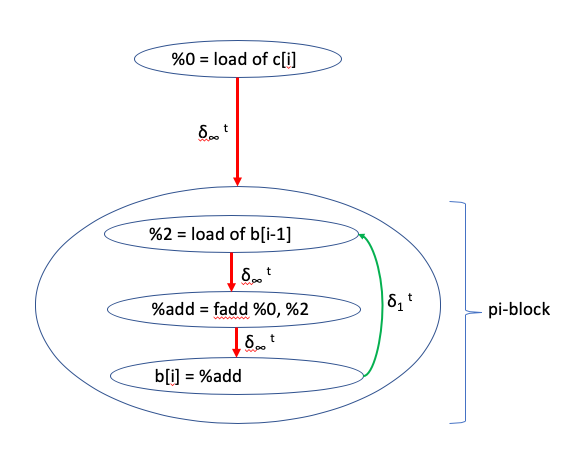
\includegraphics[width=0.55\textwidth]{figures/cycle_pi.png}
  \end{figure}
\end{frame}

\begin{frame}[label=DDGLLVM]{Data Dependence Graphs in LLVM}
  \begin{itemize}
  \item Directed Graph: D64088 (base class for various dependence graphs)
  \item Data Dependence Graph (DDG): D65350 (basic framework), D67970 (root-node), ...  
  \item Program Dependence Graph (PDG): will follow after DDG (leverage common graph builder)
  \item Envisioned Consumers:
    \begin{itemize}
    \item Loop Fusion
    \item Loop Fission
    \end{itemize}
  \end{itemize}
\end{frame}

\end{document}
